\documentclass[twoside]{book}

% Packages required by doxygen
\usepackage{fixltx2e}
\usepackage{calc}
\usepackage{doxygen}
\usepackage[export]{adjustbox} % also loads graphicx
\usepackage{graphicx}
\usepackage[utf8]{inputenc}
\usepackage{makeidx}
\usepackage{multicol}
\usepackage{multirow}
\PassOptionsToPackage{warn}{textcomp}
\usepackage{textcomp}
\usepackage[nointegrals]{wasysym}
\usepackage[table]{xcolor}

% Font selection
\usepackage[T1]{fontenc}
\usepackage[scaled=.90]{helvet}
\usepackage{courier}
\usepackage{amssymb}
\usepackage{sectsty}
\renewcommand{\familydefault}{\sfdefault}
\allsectionsfont{%
  \fontseries{bc}\selectfont%
  \color{darkgray}%
}
\renewcommand{\DoxyLabelFont}{%
  \fontseries{bc}\selectfont%
  \color{darkgray}%
}
\newcommand{\+}{\discretionary{\mbox{\scriptsize$\hookleftarrow$}}{}{}}

% Page & text layout
\usepackage{geometry}
\geometry{%
  a4paper,%
  top=2.5cm,%
  bottom=2.5cm,%
  left=2.5cm,%
  right=2.5cm%
}
\tolerance=750
\hfuzz=15pt
\hbadness=750
\setlength{\emergencystretch}{15pt}
\setlength{\parindent}{0cm}
\setlength{\parskip}{3ex plus 2ex minus 2ex}
\makeatletter
\renewcommand{\paragraph}{%
  \@startsection{paragraph}{4}{0ex}{-1.0ex}{1.0ex}{%
    \normalfont\normalsize\bfseries\SS@parafont%
  }%
}
\renewcommand{\subparagraph}{%
  \@startsection{subparagraph}{5}{0ex}{-1.0ex}{1.0ex}{%
    \normalfont\normalsize\bfseries\SS@subparafont%
  }%
}
\makeatother

% Headers & footers
\usepackage{fancyhdr}
\pagestyle{fancyplain}
\fancyhead[LE]{\fancyplain{}{\bfseries\thepage}}
\fancyhead[CE]{\fancyplain{}{}}
\fancyhead[RE]{\fancyplain{}{\bfseries\leftmark}}
\fancyhead[LO]{\fancyplain{}{\bfseries\rightmark}}
\fancyhead[CO]{\fancyplain{}{}}
\fancyhead[RO]{\fancyplain{}{\bfseries\thepage}}
\fancyfoot[LE]{\fancyplain{}{}}
\fancyfoot[CE]{\fancyplain{}{}}
\fancyfoot[RE]{\fancyplain{}{\bfseries\scriptsize Generated by Doxygen }}
\fancyfoot[LO]{\fancyplain{}{\bfseries\scriptsize Generated by Doxygen }}
\fancyfoot[CO]{\fancyplain{}{}}
\fancyfoot[RO]{\fancyplain{}{}}
\renewcommand{\footrulewidth}{0.4pt}
\renewcommand{\chaptermark}[1]{%
  \markboth{#1}{}%
}
\renewcommand{\sectionmark}[1]{%
  \markright{\thesection\ #1}%
}

% Indices & bibliography
\usepackage{natbib}
\usepackage[titles]{tocloft}
\setcounter{tocdepth}{3}
\setcounter{secnumdepth}{5}
\makeindex

% Hyperlinks (required, but should be loaded last)
\usepackage{ifpdf}
\ifpdf
  \usepackage[pdftex,pagebackref=true]{hyperref}
\else
  \usepackage[ps2pdf,pagebackref=true]{hyperref}
\fi
\hypersetup{%
  colorlinks=true,%
  linkcolor=blue,%
  citecolor=blue,%
  unicode%
}

% Custom commands
\newcommand{\clearemptydoublepage}{%
  \newpage{\pagestyle{empty}\cleardoublepage}%
}

\usepackage{caption}
\captionsetup{labelsep=space,justification=centering,font={bf},singlelinecheck=off,skip=4pt,position=top}

%===== C O N T E N T S =====

\begin{document}

% Titlepage & ToC
\hypersetup{pageanchor=false,
             bookmarksnumbered=true,
             pdfencoding=unicode
            }
\pagenumbering{roman}
\begin{titlepage}
\vspace*{7cm}
\begin{center}%
{\Large print\+\_\+ip }\\
\vspace*{1cm}
{\large Generated by Doxygen 1.8.11}\\
\end{center}
\end{titlepage}
\clearemptydoublepage
\tableofcontents
\clearemptydoublepage
\pagenumbering{arabic}
\hypersetup{pageanchor=true}

%--- Begin generated contents ---
\chapter{Module Index}
\section{Modules}
Here is a list of all modules\+:\begin{DoxyCompactList}
\item \contentsline{section}{Helpers}{\pageref{group__helpers}}{}
\end{DoxyCompactList}

\chapter{Class Index}
\section{Class List}
Here are the classes, structs, unions and interfaces with brief descriptions\+:\begin{DoxyCompactList}
\item\contentsline{section}{\hyperlink{structprint__tuple__elements}{print\+\_\+tuple\+\_\+elements$<$ index, Head, Args $>$} }{\pageref{structprint__tuple__elements}}{}
\item\contentsline{section}{\hyperlink{structprint__tuple__elements_3_010_00_01_head_00_01_args_8_8_8_01_4}{print\+\_\+tuple\+\_\+elements$<$ 0, Head, Args... $>$} }{\pageref{structprint__tuple__elements_3_010_00_01_head_00_01_args_8_8_8_01_4}}{}
\end{DoxyCompactList}

\chapter{File Index}
\section{File List}
Here is a list of all files with brief descriptions\+:\begin{DoxyCompactList}
\item\contentsline{section}{\hyperlink{main_8cpp}{main.\+cpp} }{\pageref{main_8cpp}}{}
\end{DoxyCompactList}

\chapter{Module Documentation}
\hypertarget{group__helpers}{}\section{Helpers}
\label{group__helpers}\index{Helpers@{Helpers}}
\subsection*{Classes}
\begin{DoxyCompactItemize}
\item 
struct \hyperlink{structprint__tuple__elements}{print\+\_\+tuple\+\_\+elements$<$ index, Head, Args $>$}
\item 
struct \hyperlink{structprint__tuple__elements_3_010_00_01_head_00_01_args_8_8_8_01_4}{print\+\_\+tuple\+\_\+elements$<$ 0, Head, Args... $>$}
\end{DoxyCompactItemize}


\subsection{Detailed Description}
Helpers for tuple printer. 
\chapter{Class Documentation}
\hypertarget{structprint__tuple__elements}{}\section{print\+\_\+tuple\+\_\+elements$<$ index, Head, Args $>$ Struct Template Reference}
\label{structprint__tuple__elements}\index{print\+\_\+tuple\+\_\+elements$<$ index, Head, Args $>$@{print\+\_\+tuple\+\_\+elements$<$ index, Head, Args $>$}}
\subsection*{Static Public Member Functions}
\begin{DoxyCompactItemize}
\item 
static void \hyperlink{structprint__tuple__elements_a9ea727ab1cbe97a11f82fff8b88f7811}{print} (const std\+::tuple$<$ Head, Args... $>$ \&tup)
\end{DoxyCompactItemize}


\subsection{Member Function Documentation}
\index{print\+\_\+tuple\+\_\+elements@{print\+\_\+tuple\+\_\+elements}!print@{print}}
\index{print@{print}!print\+\_\+tuple\+\_\+elements@{print\+\_\+tuple\+\_\+elements}}
\subsubsection[{\texorpdfstring{print(const std\+::tuple$<$ Head, Args... $>$ \&tup)}{print(const std::tuple< Head, Args... > &tup)}}]{\setlength{\rightskip}{0pt plus 5cm}template$<$size\+\_\+t index, typename Head , typename... Args$>$ static void {\bf print\+\_\+tuple\+\_\+elements}$<$ index, Head, Args $>$\+::print (
\begin{DoxyParamCaption}
\item[{const std\+::tuple$<$ Head, Args... $>$ \&}]{tup}
\end{DoxyParamCaption}
)\hspace{0.3cm}{\ttfamily [inline]}, {\ttfamily [static]}}\hypertarget{structprint__tuple__elements_a9ea727ab1cbe97a11f82fff8b88f7811}{}\label{structprint__tuple__elements_a9ea727ab1cbe97a11f82fff8b88f7811}


The documentation for this struct was generated from the following file\+:\begin{DoxyCompactItemize}
\item 
\hyperlink{main_8cpp}{main.\+cpp}\end{DoxyCompactItemize}

\hypertarget{structprint__tuple__elements_3_010_00_01_head_00_01_args_8_8_8_01_4}{}\section{print\+\_\+tuple\+\_\+elements$<$ 0, Head, Args... $>$ Struct Template Reference}
\label{structprint__tuple__elements_3_010_00_01_head_00_01_args_8_8_8_01_4}\index{print\+\_\+tuple\+\_\+elements$<$ 0, Head, Args... $>$@{print\+\_\+tuple\+\_\+elements$<$ 0, Head, Args... $>$}}
\subsection*{Static Public Member Functions}
\begin{DoxyCompactItemize}
\item 
static void \hyperlink{structprint__tuple__elements_3_010_00_01_head_00_01_args_8_8_8_01_4_ae87847b7f14326b50566767ca4ddad32}{print} (const std\+::tuple$<$ Head, Args... $>$ \&tup)
\end{DoxyCompactItemize}


\subsection{Member Function Documentation}
\index{print\+\_\+tuple\+\_\+elements$<$ 0, Head, Args... $>$@{print\+\_\+tuple\+\_\+elements$<$ 0, Head, Args... $>$}!print@{print}}
\index{print@{print}!print\+\_\+tuple\+\_\+elements$<$ 0, Head, Args... $>$@{print\+\_\+tuple\+\_\+elements$<$ 0, Head, Args... $>$}}
\subsubsection[{\texorpdfstring{print(const std\+::tuple$<$ Head, Args... $>$ \&tup)}{print(const std::tuple< Head, Args... > &tup)}}]{\setlength{\rightskip}{0pt plus 5cm}template$<$typename Head , typename... Args$>$ static void {\bf print\+\_\+tuple\+\_\+elements}$<$ 0, Head, Args... $>$\+::print (
\begin{DoxyParamCaption}
\item[{const std\+::tuple$<$ Head, Args... $>$ \&}]{tup}
\end{DoxyParamCaption}
)\hspace{0.3cm}{\ttfamily [inline]}, {\ttfamily [static]}}\hypertarget{structprint__tuple__elements_3_010_00_01_head_00_01_args_8_8_8_01_4_ae87847b7f14326b50566767ca4ddad32}{}\label{structprint__tuple__elements_3_010_00_01_head_00_01_args_8_8_8_01_4_ae87847b7f14326b50566767ca4ddad32}


The documentation for this struct was generated from the following file\+:\begin{DoxyCompactItemize}
\item 
\hyperlink{main_8cpp}{main.\+cpp}\end{DoxyCompactItemize}

\chapter{File Documentation}
\hypertarget{_c_make_cache_8txt}{}\section{C\+Make\+Cache.\+txt File Reference}
\label{_c_make_cache_8txt}\index{C\+Make\+Cache.\+txt@{C\+Make\+Cache.\+txt}}

\hypertarget{_c_make_lists_8txt}{}\section{C\+Make\+Lists.\+txt File Reference}
\label{_c_make_lists_8txt}\index{C\+Make\+Lists.\+txt@{C\+Make\+Lists.\+txt}}
\subsection*{Functions}
\begin{DoxyCompactItemize}
\item 
\hyperlink{_c_make_lists_8txt_a5aaac8b14fdd873a557bf67e55305bfb}{cmake\+\_\+minimum\+\_\+required} (V\+E\+R\+S\+I\+ON 3.\+2) if(\$E\+NV
\item 
\hyperlink{_c_make_lists_8txt_a54a39959e2e50a3aa543e0c203d3ff14}{set} (V\+E\+R\+S\+I\+ON 0.\+0.\$E\+NV\{T\+R\+A\+V\+I\+S\+\_\+\+B\+U\+I\+L\+D\+\_\+\+N\+U\+M\+B\+ER\}) else() set(V\+E\+R\+S\+I\+ON 0.\+0.\+0) endif() project(\hyperlink{main_8cpp_a7035d809552e6b68035896f4c083ce6b}{print\+\_\+ip} V\+E\+R\+S\+I\+ON \$
\end{DoxyCompactItemize}


\subsection{Function Documentation}
\index{C\+Make\+Lists.\+txt@{C\+Make\+Lists.\+txt}!cmake\+\_\+minimum\+\_\+required@{cmake\+\_\+minimum\+\_\+required}}
\index{cmake\+\_\+minimum\+\_\+required@{cmake\+\_\+minimum\+\_\+required}!C\+Make\+Lists.\+txt@{C\+Make\+Lists.\+txt}}
\subsubsection[{\texorpdfstring{cmake\+\_\+minimum\+\_\+required(\+V\+E\+R\+S\+I\+O\+N 3.\+2) if(\$\+E\+NV}{cmake_minimum_required(VERSION 3.2) if($ENV}}]{\setlength{\rightskip}{0pt plus 5cm}cmake\+\_\+minimum\+\_\+required (
\begin{DoxyParamCaption}
\item[{V\+E\+R\+S\+I\+ON 3.}]{2}
\end{DoxyParamCaption}
)}\hypertarget{_c_make_lists_8txt_a5aaac8b14fdd873a557bf67e55305bfb}{}\label{_c_make_lists_8txt_a5aaac8b14fdd873a557bf67e55305bfb}
\index{C\+Make\+Lists.\+txt@{C\+Make\+Lists.\+txt}!set@{set}}
\index{set@{set}!C\+Make\+Lists.\+txt@{C\+Make\+Lists.\+txt}}
\subsubsection[{\texorpdfstring{set(\+V\+E\+R\+S\+I\+O\+N 0.\+0.\$\+E\+NV\lcurly{}T\+R\+A\+V\+I\+S\+\_\+\+B\+U\+I\+L\+D\+\_\+\+N\+U\+M\+B\+ER\rcurly{}) else() set(\+V\+E\+R\+S\+I\+O\+N 0.\+0.\+0) endif() project(print\+\_\+ip V\+E\+R\+S\+I\+O\+N \$}{set(VERSION 0.0.$ENV\{TRAVIS_BUILD_NUMBER\}) else() set(VERSION 0.0.0) endif() project(print_ip VERSION $}}]{\setlength{\rightskip}{0pt plus 5cm}set (
\begin{DoxyParamCaption}
\item[{V\+E\+R\+S\+I\+ON 0.\+0.\$E\+NV\{T\+R\+A\+V\+I\+S\+\_\+\+B\+U\+I\+L\+D\+\_\+\+N\+U\+M\+B\+ER\}}]{}
\end{DoxyParamCaption}
)}\hypertarget{_c_make_lists_8txt_a54a39959e2e50a3aa543e0c203d3ff14}{}\label{_c_make_lists_8txt_a54a39959e2e50a3aa543e0c203d3ff14}

\hypertarget{install__manifest_8txt}{}\section{install\+\_\+manifest.\+txt File Reference}
\label{install__manifest_8txt}\index{install\+\_\+manifest.\+txt@{install\+\_\+manifest.\+txt}}

\hypertarget{main_8cpp}{}\section{main.\+cpp File Reference}
\label{main_8cpp}\index{main.\+cpp@{main.\+cpp}}
{\ttfamily \#include $<$list$>$}\\*
{\ttfamily \#include $<$tuple$>$}\\*
{\ttfamily \#include $<$vector$>$}\\*
{\ttfamily \#include $<$bitset$>$}\\*
{\ttfamily \#include $<$iostream$>$}\\*
{\ttfamily \#include $<$type\+\_\+traits$>$}\\*
Include dependency graph for main.\+cpp\+:
\nopagebreak
\begin{figure}[H]
\begin{center}
\leavevmode
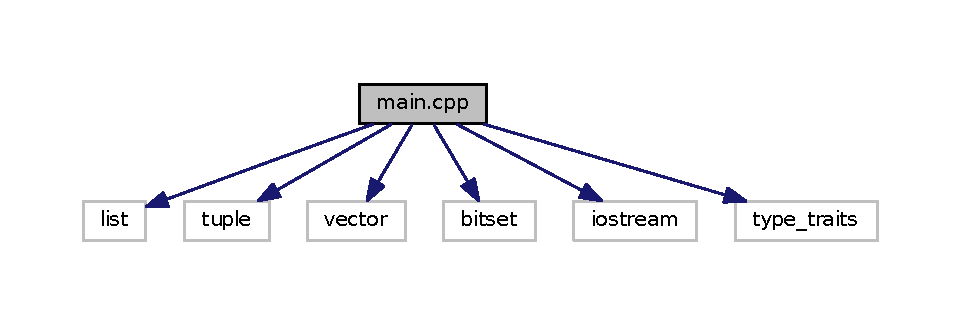
\includegraphics[width=350pt]{main_8cpp__incl}
\end{center}
\end{figure}
\subsection*{Classes}
\begin{DoxyCompactItemize}
\item 
struct \hyperlink{structprint__tuple__elements}{print\+\_\+tuple\+\_\+elements$<$ index, Head, Args $>$}
\item 
struct \hyperlink{structprint__tuple__elements_3_010_00_01_head_00_01_args_8_8_8_01_4}{print\+\_\+tuple\+\_\+elements$<$ 0, Head, Args... $>$}
\end{DoxyCompactItemize}
\subsection*{Functions}
\begin{DoxyCompactItemize}
\item 
{\footnotesize template$<$typename T , typename  = std\+::enable\+\_\+if\+\_\+t$<$std\+::is\+\_\+integral\+\_\+v$<$\+T$>$$>$$>$ }\\void \hyperlink{main_8cpp_ab0ee94f0f283926675c2820c1e63c9e3}{print} (T val)
\begin{DoxyCompactList}\small\item\em Prints ip address as integer value. \end{DoxyCompactList}\item 
{\footnotesize template$<$typename T , typename  = std\+::enable\+\_\+if\+\_\+t$<$std\+::is\+\_\+same\+\_\+v$<$\+T, std\+::string$>$$>$$>$ }\\void \hyperlink{main_8cpp_add22f80e675a041f07648b701fc81b88}{print} (const T \&val)
\begin{DoxyCompactList}\small\item\em Prints ip address as string value. \end{DoxyCompactList}\item 
{\footnotesize template$<$template$<$ typename... $>$ typename T, typename... Args, typename  = std\+::enable\+\_\+if\+\_\+t $<$		std\+::is\+\_\+same\+\_\+v		$<$			\+T$<$\+Args...$>$,			std\+::vector$<$\+Args...$>$		$>$		$\vert$$\vert$		std\+::is\+\_\+same\+\_\+v		$<$			\+T$<$\+Args...$>$,			std\+::list$<$\+Args...$>$		$>$	$>$$>$ }\\void \hyperlink{main_8cpp_aa493d86bff454f600112ae8ce5d4a76d}{print} (const T$<$ Args... $>$ \&container)
\begin{DoxyCompactList}\small\item\em Prints ip address as container (vector or list) value. \end{DoxyCompactList}\item 
{\footnotesize template$<$template$<$ typename... $>$ typename T, typename Head , typename... Args, typename  = std\+::enable\+\_\+if\+\_\+t $<$ 			std\+::is\+\_\+same\+\_\+v			$<$ 				\+T$<$\+Head, Args...$>$,				std\+::tuple$<$\+Head, Args...$>$			$>$			\&\&			(std\+::is\+\_\+same\+\_\+v$<$\+Head, Args$>$ \&\& ...)	$>$$>$ }\\void \hyperlink{main_8cpp_a9c57fe1bf9672697161c72eafc9fb786}{print} (const T$<$ Head, Args... $>$ \&tup)
\begin{DoxyCompactList}\small\item\em Prints ip address as tuple value. \end{DoxyCompactList}\item 
{\footnotesize template$<$typename T $>$ }\\void \hyperlink{main_8cpp_a7035d809552e6b68035896f4c083ce6b}{print\+\_\+ip} (const T \&val)
\begin{DoxyCompactList}\small\item\em Function wraper for all printers. \end{DoxyCompactList}\item 
int \hyperlink{main_8cpp_ae66f6b31b5ad750f1fe042a706a4e3d4}{main} ()
\begin{DoxyCompactList}\small\item\em Main function. \end{DoxyCompactList}\end{DoxyCompactItemize}


\subsection{Function Documentation}
\index{main.\+cpp@{main.\+cpp}!main@{main}}
\index{main@{main}!main.\+cpp@{main.\+cpp}}
\subsubsection[{\texorpdfstring{main()}{main()}}]{\setlength{\rightskip}{0pt plus 5cm}int main (
\begin{DoxyParamCaption}
{}
\end{DoxyParamCaption}
)}\hypertarget{main_8cpp_ae66f6b31b5ad750f1fe042a706a4e3d4}{}\label{main_8cpp_ae66f6b31b5ad750f1fe042a706a4e3d4}


Main function. 

\index{main.\+cpp@{main.\+cpp}!print@{print}}
\index{print@{print}!main.\+cpp@{main.\+cpp}}
\subsubsection[{\texorpdfstring{print(\+T val)}{print(T val)}}]{\setlength{\rightskip}{0pt plus 5cm}template$<$typename T , typename  = std\+::enable\+\_\+if\+\_\+t$<$std\+::is\+\_\+integral\+\_\+v$<$\+T$>$$>$$>$ void print (
\begin{DoxyParamCaption}
\item[{T}]{val}
\end{DoxyParamCaption}
)}\hypertarget{main_8cpp_ab0ee94f0f283926675c2820c1e63c9e3}{}\label{main_8cpp_ab0ee94f0f283926675c2820c1e63c9e3}


Prints ip address as integer value. 

\index{main.\+cpp@{main.\+cpp}!print@{print}}
\index{print@{print}!main.\+cpp@{main.\+cpp}}
\subsubsection[{\texorpdfstring{print(const T \&val)}{print(const T &val)}}]{\setlength{\rightskip}{0pt plus 5cm}template$<$typename T , typename  = std\+::enable\+\_\+if\+\_\+t$<$std\+::is\+\_\+same\+\_\+v$<$\+T, std\+::string$>$$>$$>$ void print (
\begin{DoxyParamCaption}
\item[{const T \&}]{val}
\end{DoxyParamCaption}
)}\hypertarget{main_8cpp_add22f80e675a041f07648b701fc81b88}{}\label{main_8cpp_add22f80e675a041f07648b701fc81b88}


Prints ip address as string value. 

\index{main.\+cpp@{main.\+cpp}!print@{print}}
\index{print@{print}!main.\+cpp@{main.\+cpp}}
\subsubsection[{\texorpdfstring{print(const T$<$ Args... $>$ \&container)}{print(const T< Args... > &container)}}]{\setlength{\rightskip}{0pt plus 5cm}template$<$template$<$ typename... $>$ typename T, typename... Args, typename  = std\+::enable\+\_\+if\+\_\+t $<$		std\+::is\+\_\+same\+\_\+v		$<$			\+T$<$\+Args...$>$,			std\+::vector$<$\+Args...$>$		$>$		$\vert$$\vert$		std\+::is\+\_\+same\+\_\+v		$<$			\+T$<$\+Args...$>$,			std\+::list$<$\+Args...$>$		$>$	$>$$>$ void print (
\begin{DoxyParamCaption}
\item[{const T$<$ Args... $>$ \&}]{container}
\end{DoxyParamCaption}
)}\hypertarget{main_8cpp_aa493d86bff454f600112ae8ce5d4a76d}{}\label{main_8cpp_aa493d86bff454f600112ae8ce5d4a76d}


Prints ip address as container (vector or list) value. 

\index{main.\+cpp@{main.\+cpp}!print@{print}}
\index{print@{print}!main.\+cpp@{main.\+cpp}}
\subsubsection[{\texorpdfstring{print(const T$<$ Head, Args... $>$ \&tup)}{print(const T< Head, Args... > &tup)}}]{\setlength{\rightskip}{0pt plus 5cm}template$<$template$<$ typename... $>$ typename T, typename Head , typename... Args, typename  = std\+::enable\+\_\+if\+\_\+t $<$ 			std\+::is\+\_\+same\+\_\+v			$<$ 				\+T$<$\+Head, Args...$>$,				std\+::tuple$<$\+Head, Args...$>$			$>$			\&\&			(std\+::is\+\_\+same\+\_\+v$<$\+Head, Args$>$ \&\& ...)	$>$$>$ void print (
\begin{DoxyParamCaption}
\item[{const T$<$ Head, Args... $>$ \&}]{tup}
\end{DoxyParamCaption}
)}\hypertarget{main_8cpp_a9c57fe1bf9672697161c72eafc9fb786}{}\label{main_8cpp_a9c57fe1bf9672697161c72eafc9fb786}


Prints ip address as tuple value. 

\index{main.\+cpp@{main.\+cpp}!print\+\_\+ip@{print\+\_\+ip}}
\index{print\+\_\+ip@{print\+\_\+ip}!main.\+cpp@{main.\+cpp}}
\subsubsection[{\texorpdfstring{print\+\_\+ip(const T \&val)}{print_ip(const T &val)}}]{\setlength{\rightskip}{0pt plus 5cm}template$<$typename T $>$ void print\+\_\+ip (
\begin{DoxyParamCaption}
\item[{const T \&}]{val}
\end{DoxyParamCaption}
)}\hypertarget{main_8cpp_a7035d809552e6b68035896f4c083ce6b}{}\label{main_8cpp_a7035d809552e6b68035896f4c083ce6b}


Function wraper for all printers. 


%--- End generated contents ---

% Index
\backmatter
\newpage
\phantomsection
\clearemptydoublepage
\addcontentsline{toc}{chapter}{Index}
\printindex

\end{document}
